\documentclass{beamer}
\usepackage[utf8]{inputenc}

\title{ Optimization}

\institute{ \large GOUTHAM A.G.V  \and EE17BTECH11001   } 

\begin{document}

\maketitle

\begin{frame}{INTRODUCTION
}


\ Problem Statement 7.8:
\begin{itemize}
\item A cooperative society
of farmers has 50 hectare of land to grow two
crops X and Y.  
\item   The profit from crops X and Y
per hectare are estimated as Rs 10,500 and Rs
9,000 respectively.
\item  To control weeds, a liquid
herbicide has to be used for crops X and Y
at rates of 20 litres and 10 litres per hectare and no more than 800 litres of herbicide
should be used
\item  How much land should be
allocated to each crop so as to maximise the
total profit of the society?

\end{itemize}
\end{frame}

\begin{frame}{Decision Variables and Objective Function}

\textbf{Decision Variables:}
\vspace{0.4cm}
\begin{itemize}
\item : $X$: Number of hectares of land in which 'x' is cultivated
\item : $Y$: Number of hectares of land in which 'y' is cultivated
\vspace{0.8cm}
\end{itemize}
\textbf{Objective Function:}\\
\vspace{0.2cm}
\begin{itemize}
\item Profit = 
\hspace{0.15cm}Profit from x per hectare * X\\
\hspace{3.3cm} \textbf{+}\\
\hspace{1.6cm} Profit from y per hectare * Y\\
\end{itemize}
\vspace{0.5cm}
\Large
$$Profit_{max} = 10500 * X + 9000 * Y$$

\end{frame}


\begin{frame}{Constraints}
% \scriptsize
\begin{equation}\label{1}
    \textbf{X + Y = 50}            
\end{equation} 
\begin{equation} 
   \textbf{20 * X + 10 * Y} <\textbf{= 800}
\end{equation}

\begin{itemize}
\item Constraint (1) indicates the total number of hectares available to cultivate both X and Y in our mission to maximise profit.
\item Constraint (2) ensures that the total amount of herbicide used for cultivating is no more than 800 litres
\end{itemize}
\end{frame}

\begin{frame}{Graph}
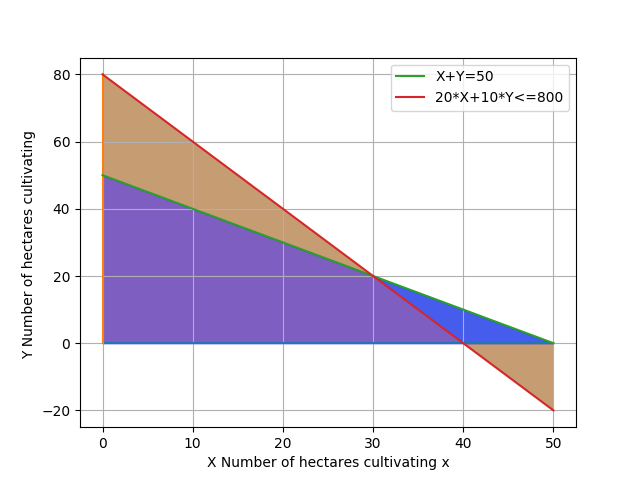
\includegraphics[scale=0.6]{Figure_1.png}
\end{frame}
\begin{frame}{Solution}

Number of hectares with x crop = 30\\
Number of hectares with y crop = 20\\
Total Profit = 495000\\
\vspace{0.3cm}
\centering{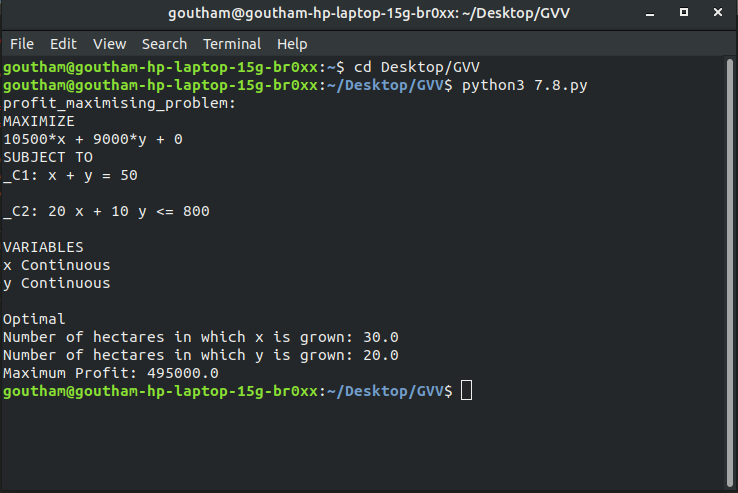
\includegraphics[scale=0.25]{a.png}\\}
\vspace{0.3cm}
\small{Code for this problem can be accessed  \href{https://github.com/gouthamagv/Optimisation_GVV/blob/master/7.8.py}{here}}

\end{frame}
\end{document}
